\exercise
Merge Sort
روش مرتب سازی ادغامی: یک روش مرتب سازی مبتنی بر مقایسه عناصر با استفاده از روش تقسیم و غلبه است. این روش از مراحل بازگشتی زیر تشکیل یافته است.

۱- آرایه را به دو زیر آرایه با اندازه تقریبا یکسان تقسیم کن.

۲-دو زیر آرایه را به روش مرتب سازی ادغامی مرتب کن.

۳- دو زیر آرایه مرتب شده را ادغام کن.

    \begin{center}
     	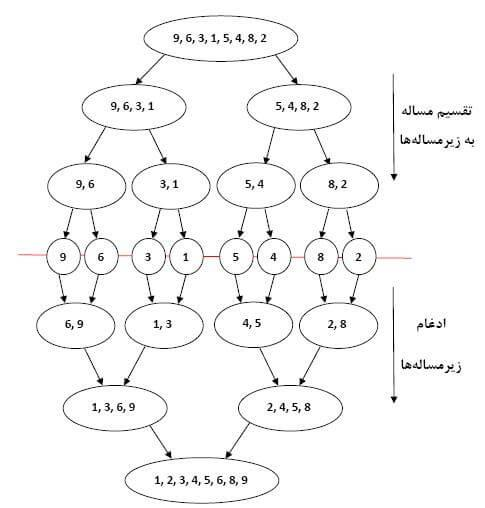
\includegraphics[scale=0.5]{./3.png}
    \end{center}

فرض کنید در الگوریتم مرتب سازی ادغامی هزینه زمان لازم برای ادغام دو آرایه هر کدام به طول
$k$
برابر
$2kt + 1$
باشد که در آن
$t$
واحد زمانی وابسته به پردازنده است (ثابت فرض شود).
$2^m$
عدد تامرتب را در نظر بگیرید که برای مرتب شدن به روش مذکور در اختیار ما قرار گرفته اند. اگر داده ها را در هر تقسیم دقیقا به دو قسمت مساوی تقسیم کنیم:

الف) رابطه بازگشتی برای محاسبه زمان اجرای الگوریتم را بدست آورید‌(برای هر مرحله ای که دو آرایه به طول 
$L$
در حال ادغام اند. زمان اجرای این مرحله را
$T(L)$
بنامید.)

ب) با استفاده از رابطه ای که بدست آوردید زمان اجرای برنامه را بر حسب
$m$
و
$t$
بدست آورید.

ج) با توجه به پاسخ قسمت (ب)و مرتبه زمانی الگوریتم را بر حسب
$n$
که
$n = 2^m$
باشد بیان کنید.

نکته) از زمان صرف شده برای تقسیم کردن آرایه صرف نظر کنید و محاسبات را از اولین گام آغاز کنید.

راهنمایی) پاسخ قسمت (الف) باید به شکل
$T(L) = f(T(g(L)))$
باشد که در آن
$g$
و
$f$
دو تابع هستند.

نکته) در قسمت های (الف) و (ج) فقط پاسخ نهایی اهمیت دارد و بررسی می شود.